% !TEX root = ../HDR.tex
%%%%%%%%%%%%%%%%%%%%%%%%%%%%%%%%%%%%%%%%%%%%%%%%%%%%%%%%%%%%%%%%%%%%%%%%%%%%%%%%%%
\chapter{Fondements en sciences cognitives}

\noindent 
Ce chapitre vise à définir l'intelligence artificielle précoce telle qu'elle est mise en oeuvre par les etres vivants, sur la base de l'épistémologie, la psychologie et les sciences cognitives. 

La finalité est de fonder un projet d'implémentation informatique qui transcrive cette vision.

\section{Épistémologie pragmatique}
\label{sec:pragmatisme}

William James: role central de l'action et de la praxis.

David Hume, Notion de \an{bundle} pour représenter les objets par l'ensemble des interactions qu'ils \an{afford}.

Ludvig Wittgenstein: \an{meaning is use} surtout connu dans le cadre de la philosophie du langage pour dire que le sens des mots provient de leur usage dans le discours. 
Mais cette pensée est plus générale pour dire que le sens de tout symbole est lié à l'usage que le sujet en fait dans le cadre de ses propres motivations. 

\section{Fondements de la connaissance dans l'habitude}

Charles Sanders Peirce est parmi les premiers à suggérer que l'apprentissage se fait par \og sédimentation d'habitudes \fg.

Cette idées est reprise en épistémologie pragmatique par David Hume: je connais le mouvement du soleil car j'ai l'habitude qu'il se lève tous les matins. 

\section{Théorie évolutionniste de la connaissance}

\begin{quote}
	\og La connaissance précède l'observation. 
	Tout animal naît avec des attentes ou anticipations qu'on pourrait reconstruire sous la forme d'hypothèses. 
	En ce sens nous disposons d'un certain degré de connaissance innée. 
	Elles seront, si elles sont désavouées, nos premiers problèmes. \fg 
	\cite[p.~389]{popper_connaissance_1979}
\end{quote}

\noindent
En affirmant que l'observation suppose toujours une connaissance préalable, mais que cette connaissance découle elle-même de l'observation, Karl Popper met en lumière une circularité qui fonde sa théorie évolutionniste de la connaissance. 
Etant issue de l’observation, la connaissance ne peut jamais être acquise comme vraie en un sens absolu. 
D'une part, toute observation est toujours biaisée par une connaissance antérieure. 
D'autre part, rien ne permet d’affirmer qu'aucun contre-exemple ne viendra jamais la réfuter. 
Dès lors, propose Popper, toute connaissance ne peut, au mieux, qu’être retenue comme acceptable aussi longtemps qu’elle n’a pas été réfutée. 
Pour lui, ce processus de \og sélection naturelle \fg des connaissances par leur réfutation constitue la seule voie permettant de tendre vers une connaissance objective du monde. 
Lorsqu'une connaissance est rejetée, elle appelle la conception d’une nouvelle connaissance plus englobante. 
C’est ainsi qu’il cite le physicien John Wheeler : \og Tout notre problème est de commettre les erreurs le plus vite possible \fg \cite{popper_connaissance_1979}.

L'approche popperienne de la connaissance a été critiquée, d'une part parce que le critère de réfutabilité s'avère souvent difficile à mettre en place, et d'autre part parce qu'elle n'explique pas le fonctionnement de l'induction, sans laquelle la création de nouvelle connaissance n'apparait possible.
Popper s'intéresse avant tout à la construction de connaissances scientifiques, en considérant le sujet connaissant (le chercheur), comme donné a priori, et déjà capable de formuler des hypothèses et d'évaluer les résultats expérimentaux à l'aune d'une théorie. 
Ce présupposé a ouvert la voie à ses successeurs, qui ont entrepris de développer une théorie de l'émergence du sujet connaissant sans postuler son existence préalable. 

Malgré ces critiques, je retiens le critère popperien de résistance à la réfutabilité dans le cadre de la conception d'agents artificiels capables d'apprentissage autonome.
Il s'agit pour l'agent artificiel de sélectionner les meilleurs éléments explicatifs élémentaires parmi une grande quantité de candidats créés, et de les traiter comme des micro-hypothèses pour construire sa connaissance à partir de son expérience.
L'agent artificiel devra mettre en œuvre des boucle de production/réfutation d'hypothèses efficaces pour répondre au problème de Wheeler.



\section{Epistémologie génétique}
\label{sec:epistemologie_genetique}

\noindent
Jean Piaget a intégré la dimension évolutionniste popperienne de la connaissance dans son \emph{Epistémologie génétique} \cite{piaget_lepistemologie_1970}.
Le terme \og génétique \fg doit s'entendre en référence à la \og genèse de la connaissance \fg au cours du développement ontogénétique du sujet connaissant.
Vers la fin de sa vie, Piaget rapprochera l'épistémologie génétique de l'épisétémologie constructiviste théorisée par d'autres auteurs comme Ernst von Galsersfeld \cite{von_glasersfeld_radical_1995}. 
Selon Piaget, le point de départ de toute connaissance est \og l'expérience vécue \fg:

\begin{quote}
	\og La connaissance ne procède en ses sources ni d’un sujet conscient de lui-même ni d’objets déjà constitués (du point de vue du sujet) qui s’imposeraient à lui : elle résulte d’interactions se produisant à mi-chemin entre les deux et relevant donc des deux à la fois, mais en raison d’une indifférenciation complète et non pas d’échanges entre formes distinctes. [...]  
	S’il n’existe au début ni sujet, au sens épistémique du terme, ni objets conçus comme tels, ni surtout d’instruments invariants d’échange, le problème initial de la connaissance sera donc de construire de tels médiateurs: partant de la zone de contact entre le corps propre et les choses, il s’engageront alors toujours plus avant dans les deux directions complémentaires de l’extérieur et de l’intérieur et c’est de cette double construction progressive que dépend l’élaboration solidaire du sujet et des objets. \fg
	\cite[p.~14]{piaget_lepistemologie_1970}
\end{quote}


Piaget part d'une hypothèse phénoménologique dans laquelle l'expérience d'interaction est centrale. 
Grâce à l'interaction répétée du corps avec son environnement, se développent des unités élémentaires de l’activité mentale, qu'il appelle \emph{schèmes}. 
Un schème est une entité abstraite qui organise l'interaction du corps avec son environnement. 
Ces schèmes s'ancrent dans l'esprit lorsque l'expérience les conforte, ou se modifient lorsque l'expérience les contredit. 
Si l'épistémologie génétique est surtout connue dans le cadre du développement de l'enfant, elle continue à s'appliquer aux apprentissage qui accompagnent la pratique d'activités nouvelles tout au long de la vie.  
Vermersch \cite{vermersch_problematique_2014} résume cet apprentissage en quatre étapes: 

\begin{enumerate}%[itemsep=0pt, parsep=0pt, partopsep=0pt]
	\item Vécu singuler inscrit dans l'action, connaissance en actes.
	\item Vécu représenté, signifants intériorisés, privés.
	\item Vécu verbalisé, habillage par les significations.
	\item Vécu comme objet de connaissance, construction de connaissance.
\end{enumerate}

En partant d'une nouvelle activité vécue par le sujet sur la base de ses connaissances antérieures qui lui permettent d'interagir avec son environnement (étape 1), le sujet construit et sélectionne de nouveaux schèmes d'interaction qui deviendront porteurs de sens dans le contexte de cette nouvelle activité (étape 2). 
Ces schèmes pourront être verbalisés et confrontés aux catégories proposées par la communauté humaine pratiquant cette activité (étape 3). 
La connaissance ainsi abstraite pourra faire l’objet d’une analyse réflexive par le sujet qui pourra prendre cette activité comme un nouvel objet de connaissance (étape 4).

Les détracteurs de l'épistémologie génétique ont contesté le rôle fondamental que Piaget donnait à l'expérience sensorimotrice.
Leurs critiques convergent avec des travaux récents suggérant l'existence d'une forme de subjectivité durant les stades tardifs de la vie intra utérine quand les apports sensorimoteurs semblent encore très limités \cite{moser_magnetoencephalographic_2021}.
On peut toutefois contre-argumenter que, même in utero, la vie fœtale n'est pas dénuée d'interactions. 
Même si Piaget semblait penser que le sujet se construisait par interaction avec le monde extérieure après la naissance, ses idées épistémologiques restent applicables aux interactions intra utérine du foetus. 
Quoi qu'il en soit, l'épistémologie génétique est largement acceptée comme la référence fondatrice des théories cherchant à expliquer l'émergence de la connaissance à parti de la matière chimique et organique. 

Je retiens le concept clé de \emph{schème sensorimoteur} comme construit cognitif qui organise l'expérience d'interaction entre le corps et l'environnement.
Un schème sensorimoteur opère comme un médiateur au sein du couplage corps/environnement.
%, à partir duquel la perception des objets extérieurs peut se construire
Piaget nous conduit à effectuer une forme d'inversion du raisonnement pour aller de l'interaction vers la perception et l'action plutôt que l'inverse:
les schèmes ne sont pas constitués d'associations de perceptions et d'actions initialement distinctes, mais ils précèdent la possibilité de percevoir le monde et d'effectuer des actions intentionnelles sur lui. 

\section{Psychologie développementale}

\noindent
Parallèlement à l'épistémologie génétique, Piaget a fondé le champ de la \emph{psychologie développementale}. 
Au-delà des dimensions théoriques de la construction du sujet connaissant, la psychologie développementale tente de décrire et comprendre le cheminement chronologique qui conduit l'esprit humain depuis l'état du nouveau-né jusqu'à celui de l'âge adulte.
Elle offre un pendant expérimental à l'épistémologie génétique, en s'appuyant sur des observations, permettant l'expérimentation, et proposant des applications. 
Dans son ouvrage \emph{Pour comprendre Jean Piagiet} \cite{dolle_pour_1997}, Jean-Marie Dolle synthétise ainsi les stades chronologiques du développement cognitif de l'être humain :

\begin{enumerate}[itemsep=0pt, parsep=0pt, partopsep=0pt]
	\item L'intelligence sensorimotrice
	\begin{enumerate}[itemsep=0pt, topsep=0pt, parsep=0pt, partopsep=0pt]
		\item Développement des structures sensorimotrices
		\begin{itemize}[label=\scalebox{.85}{$\diamond$}, itemsep=0pt, topsep=0pt, parsep=0pt, partopsep=0pt]
			\item Maitriser son propre dispositif
		\end{itemize}
		\item La construction du réel
		\begin{itemize}[label=\scalebox{.85}{$\diamond$}, itemsep=0pt, topsep=0pt, parsep=0pt, partopsep=0pt]
			\item La construction de l'objet permanent
			\item La constrution de l'espace sensorimoteur
			\item La construction de la causalité
			\item La construction du temps
		\end{itemize} 
	\end{enumerate} 
	\item La génèse des opérations concrêtes
	\begin{enumerate}[itemsep=0pt, topsep=0pt, parsep=0pt, partopsep=0pt]
		\item Intelligence représentative
		\item L'intelligence symbolique
		\item La mise en place des structures des opérations concrêtes
		\item L'espace
	\end{enumerate} 
	\item L'intelligence opératoire formelle 
\end{enumerate}

Depuis ce premier cadre posé par Piaget, la psychologie développementale s'est largement enrichie. 
Dans le chapitre \an{The origins and sources of action} de l'ouvrage \an{Oxford handbook of human action}, Bernhard Hommel et Birgit Elsner soulignent que, bien que les nouveaux-nés disposent déjà de capacités motrices et sensorielles, il est généralement admis qu'ils ne sont pas encore en mesure d'effectuer des actions intentionnelles \cite{hommel_acquisition_2009}. 
Ils peuvent mouvoir leur corps et percevoir des événements sensoriels, y compris des réactions (\an{feedbacks}) résultants de leurs mouvements. 
Les conséquences de leurs actions, qu'elles soient distales (visuelles ou auditives) ou proximales (tactiles, proprioceptives) sont enregistrées dès la naissance. 
Les auteurs posent la question centrale : comment passons-nous de l'état de nouveau-né agité et réceptif à celui d'agent intentionnel ? 

Ils retracent l'émergence progressive du contrôle d'action par d'expériences d'interaction qui commence par l'apprentissage de ce que nous avons la possibilité de faire. 
Pendant les 8 premiers mois de la vie, la maturation conduit à la différentiation de motifs de comportements innés pour améliorer la coordination et le contrôle du mouvement. 
Ils enregistrent les relations entre leurs mouvements et les événements se produisant dans l'environnement. 
Dès deux mois, les nouveaux nés peuvent apprendre à modifier la fréquence de succion pour obtenir certains résultats sensoriels comme entendre la voix de leur mère, voir certaines photos, ou obtenir leur lait préféré \cite{rochat_emerging_1999}
De deux à quatre mois, toutes sortes d'expérience ont montré l'habileté des enfants pour repérer des connexions entrer leurs mouvements de différentes parties du corps et la survenue d'événement favorables ou défavorables qui mettent en évidence l'acquisition d'une connaissance des relations action-effet et témoignent la capacité de se fixer un objectif de produire un certain événement et de déclencher les actions nécessaires pour le réaliser.Ils s'engagent dans des activités ludique consistant à répéter ses opérations et produisant des rires quand ils y parviennent ou une déception quand ils échouent. 
Hommel propose un modèle un deux étapes de l'acquisition d'actions volontaires : l'étape 1 consiste en l'apprentissage des contingences être les mouvements et les effets, et l'étape 2 consiste à se fixer des objectifs et utiliser cette connaissance pour les atteindre.   
Certaines expériences montrent que le cortex premoteur pourrait intégrer les actions avec leurs conséquences attendues sous forme d'une sorete de \an{pragmatic body map} \cite{schubotz_functional_2001}. 

Est-ce que les schemes sensorimoteurs contiennent aussi une information de valence affective ?
Un exemple est donné par l'expérience de Tom Becker et ses coauteurs \cite{beckers_automatic_2002} dans laquelle les sujets étaient entrainés à  répondre à un choix binaire de catégorie de mots affectivement neutres, l'une des réponses entrainant une légère décharge électrique.
Dans la phase de test, ils effectuaient la même tâche, mais avec des mots à valence affective positive ou négative. 
Comme attendu, la performance s’améliorait lorsque la valence du mot correspondait à celle de la réponse : les mots négatifs étaient traités plus rapidement avec la réponse associée au choc, tandis que l’inverse se produisait pour les mots positifs.
Les auteurs en concluent l'action acquière la valence affective de ses effets. 





\section{Théorie du processus}

\begin{quote}
\an{If we are to look for substance anywhere, I should find it in events which are in some sense the ultimate substance of nature.}
\cite{whitehead_process_1978}
\end{quote}

\textbf{}

Importance de la notion d'événements. 

Alfred North Whitehead

\section{Individuation}

\begin{quote}
Individuation is the formation or becoming of individuals. It is a primal formative activity whereas boundaries and distinctions arise without assuming any individual(s) that precede(s) them 
\cite[p.~9]{weinbaum_open_2015}.
\end{quote}

Marcel Turbiaux relate la pensée de Gilbert Simondon: 
\begin{quote}
	L’individuation doit être considérée comme résolution partielle et relative qui se manifeste dans un système recélant des potentiels et refermant une certaine incompatibilité par rapport à lui-même, incompatibilité faite de forces de tension aussi bien que d’impossibilité d’une interaction entre termes extrêmes des dimensions »  \cite[p.~102]{turbiaux_simondon_1967}
\end{quote}

D'après Weinbaum, selon Simondon, l’individu n’est plus l’élément rigide et bien défini de tradition aristotélicienne, doté de propriétés fixées une fois pour toutes, mais plutôt une entité plastique, un devenir en cours. L’état relativement stable des individus est ponctué de périodes de transformation, au cours desquelles ils peuvent changer radicalement ou se désintégrer. Chacune de ces périodes reconfigure les tensions internes actives au sein de l’individu ainsi que la manière dont elles détermineront les phases stables et les transformations futures.


\section{Neurosciences}

\subsection{Architectures cognitive}


\begin{figure}[ht]
	\centering
	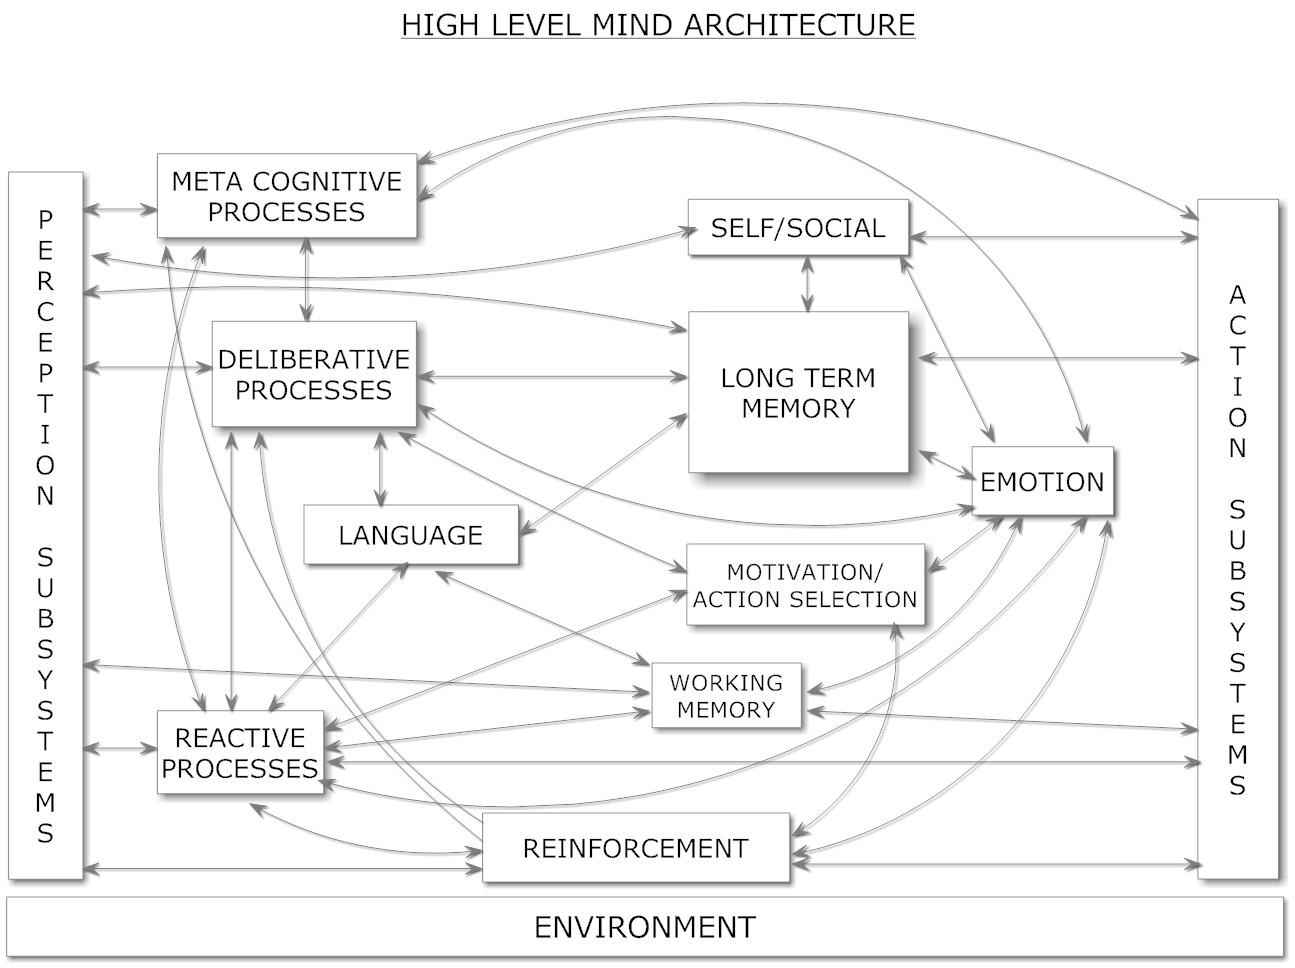
\includegraphics[width=0.7\textwidth]{Figures/1_Cognitive_architecture.png}
	\caption{Architecture cognitive de haut niveau pour une \an{human-like general intelligence} d'après Goertzel 
	\cite[Fig.~17]{goertzel_general_2021}}
	\label{fig:Cognitive_architecture}
\end{figure}

\subsection{Comportements innés}

\subsection{Emotions}

\subsection{Apprentissage spatio-sequentiel}

Roddy Grieves et Kate Jeffery font une synthèse des des connaissances sur la représentation de l'espace dans le cerveau in \ref{fig:space}.

\begin{figure}[ht]
	\centering
	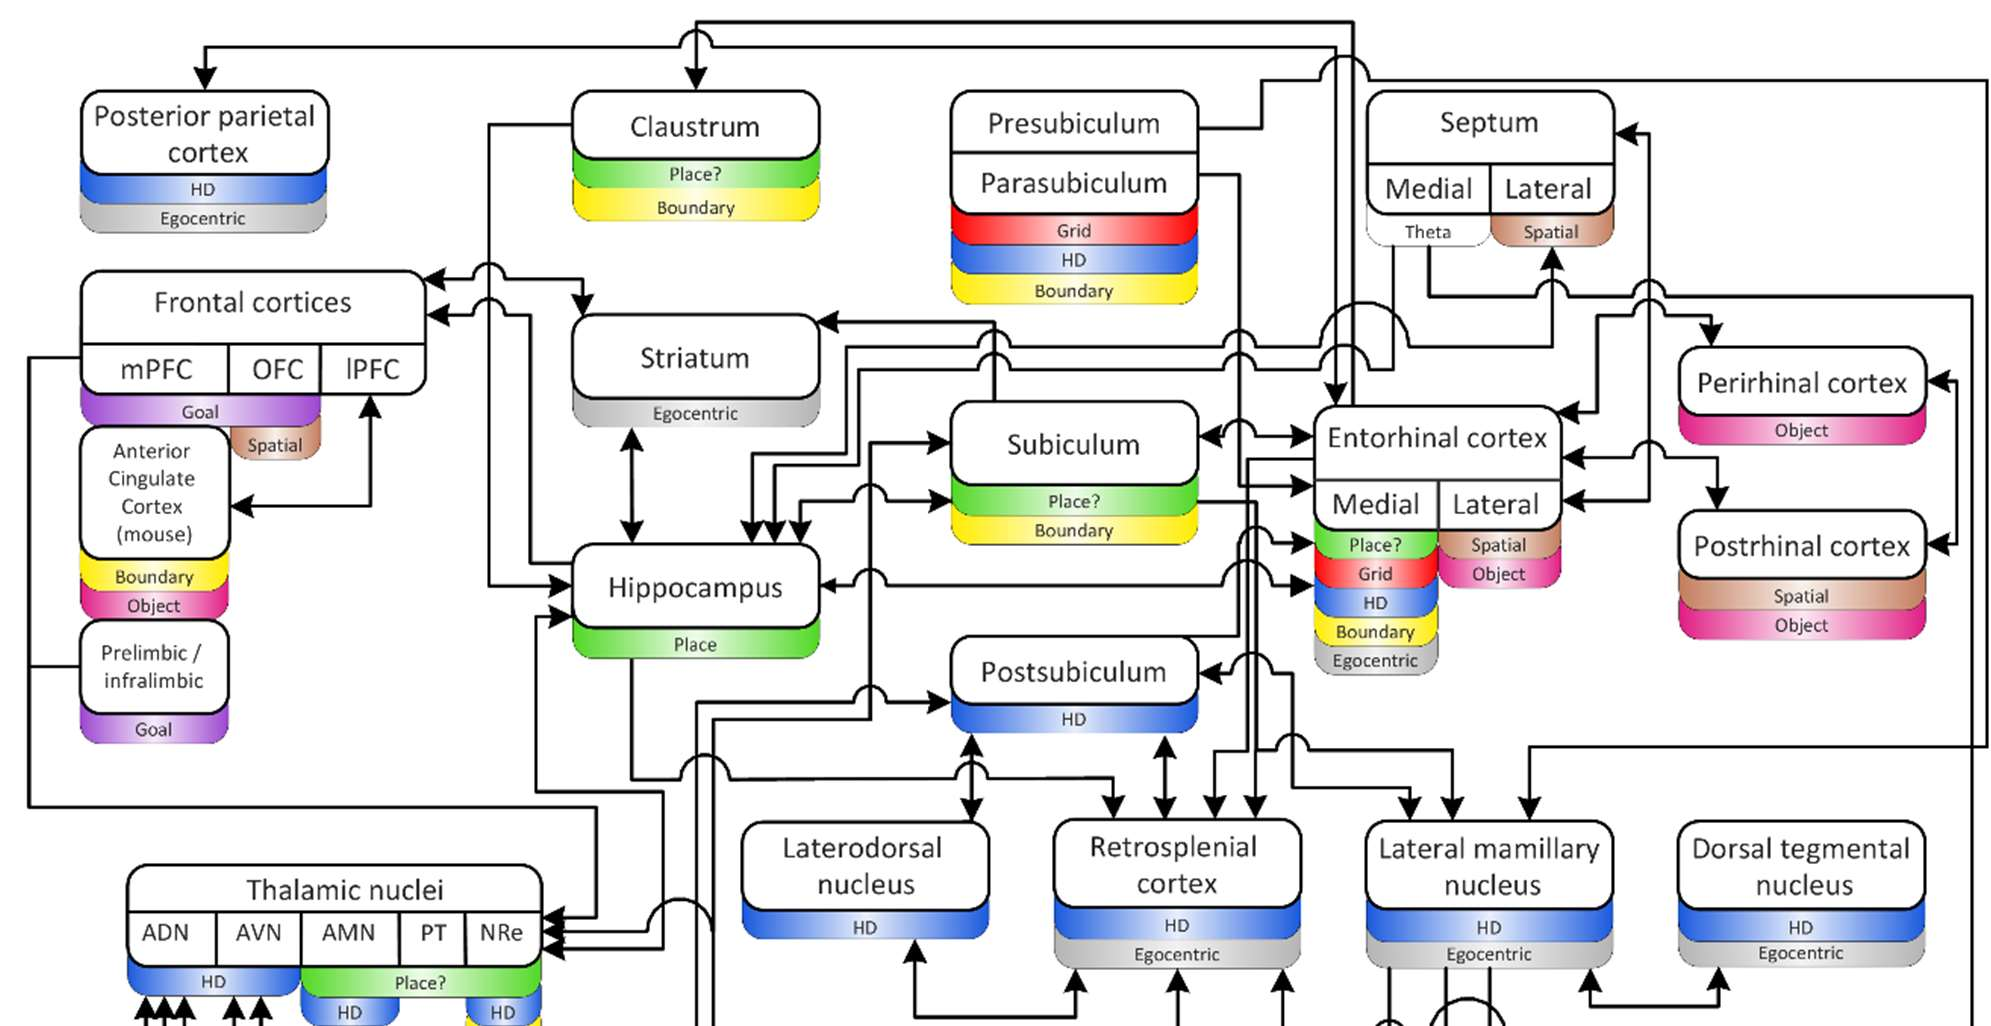
\includegraphics[width=0.7\linewidth]{Figures/1_space1.png}\\[-0.1em]
	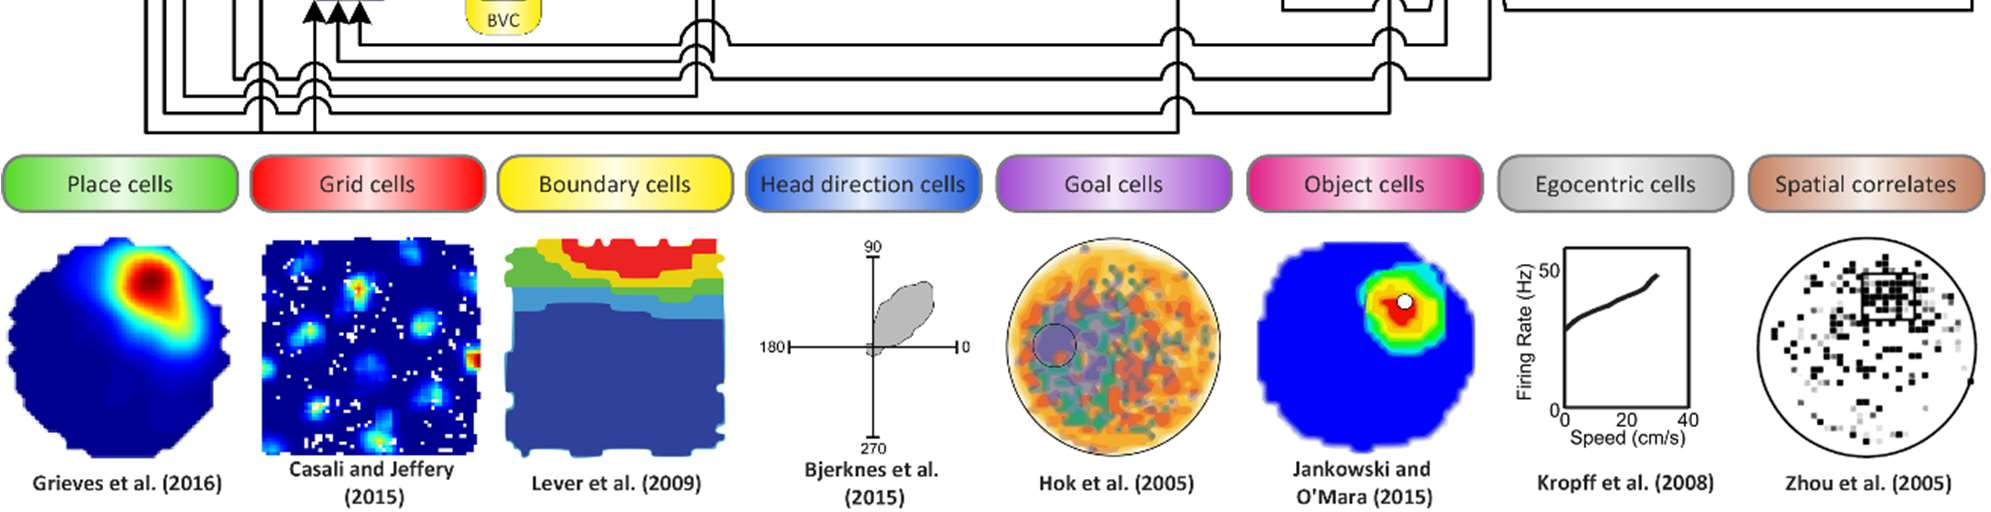
\includegraphics[width=0.7\linewidth]{Figures/1_space2.png}
	\caption{Représentation de l'espace dans le cerveau selon Grieves et Jeffery \cite[Fig.~8]{grieves_representation_2017}. 
	}
	\label{fig:space}
\end{figure}


Hippocampe: mémoire spatiale et mémoire séquentielle. 

\section{Mesures de l'intelligence}

Comment mesurer l'intelligence est une question compliquée qui n'a pas encore de réponse définitive. 
Legg note que \og \an{A fundamental problem in artificial intelligence is that nobody really knows what intelligence is} \fg \cite[p.~1]{legg_universal_2007}.

Il fait une première distinction entre les tests statiques et les testes dynamiques. 
Les tests statiques mesure la capacité de résoudre une problème présenté en une seule fois. 
Ils ne mesurent pas directemenent la capacité à apprendre et à s'adapter au cours du temps. 
Dans un test dynamique, le sujet interagit avec l'environnement de test pendant une certaine période de temps. 

Une autre distinction est selon qu'il existe une mesure de la capacité de l'agent à atteindre un objectif ou non.  
Dans le premier cas, Legg propose une mesure de l'intelligence qu'il appelle \an{universal intelligence} d'un agent qui est la somme infinie sur tous les environnements possibles dans lequel la reward est computable avec une somme bornée, de la mesure de la capacité à atteindre l'ojectif normalisée dans l'interval [0, 1] pondérée par de manière inversement proportionnelle à la complexité de l'environnement. 
Bien entendu, il n'existe pas de moyen de la calculer. 


David Deutsch exprime de manière un peu provocatrice qu'on attend d'une vraie intelligence qu'elle soit capable de désobéir: 

\begin{quote}
\an{So, despite its usefulness in other applications, the programming technique of defining a testable objective and training the program to meet it will have to be dropped. 
	Indeed, I expect that any testing in the process of creating an AGI risks being counterproductive
	%, even immoral, just as in the education of humans. 
	%I share Turing’s supposition that we’ll know an AGI when we see one, but this partial ability to recognize success won’t help in creating the successful program
	}
\cite[p.~119]{deutsch_beyond_2019}.
\end{quote}

\subsection{Abstract Reasoning Challenge}

L'objectif du \an{Abstract Reasoning Challenge} (ARC) est d'évaluer la capacité à utiliser uniquement un socle de connaissance que tout enfant ou agent naturellement intelligent est censé posséder pour résoudre des taches nouvelles, sans faire appel à des savoirs scolaires, linguistiques, ou culturels. 


Francois Cholet identifie 4 \an{core knowledge} : 

\begin{itemize}[label=\scalebox{.85}{$\diamond$}]
	\item Géométrie élémentaire, spatialisation: reconnaitre et manipuler des formes simples (lignes, rectangles, triangules, cercles). Différentier les formes même après des transformations (rotation, translation, symétrie, déformation). Détecter les positions et distances. 
	\item Objets et leur persistance: Les objets existent de manière continue ; ils ne peuvent pas apparaître ou disparaître sans raison; ils peuvent interagir selon les circonstances
	\item Nombres et comptage: il est possible de compter des petits nombres d'objets ou propriétés, et former des groupes dénombrés.
	\item Agentivité : certains objets peuvent être identifiés comme \og agents \fg poursuivant une intention ou un but. On distingue les objets animés et inanimés.
\end{itemize}

La Fig. \ref{fig:ARC} montre un exemple de problème du ARC Challenge mettant en jeu le \an{core knowledge} d'agentivité.
Dans cet exemple, la règle à inférer pour passer de l'image de gauche à celle de droite est qu'un agent se déplace d'un point à un autre en tournant quand il arrive face à un carré vert. 

\begin{figure}[ht]
	\centering
	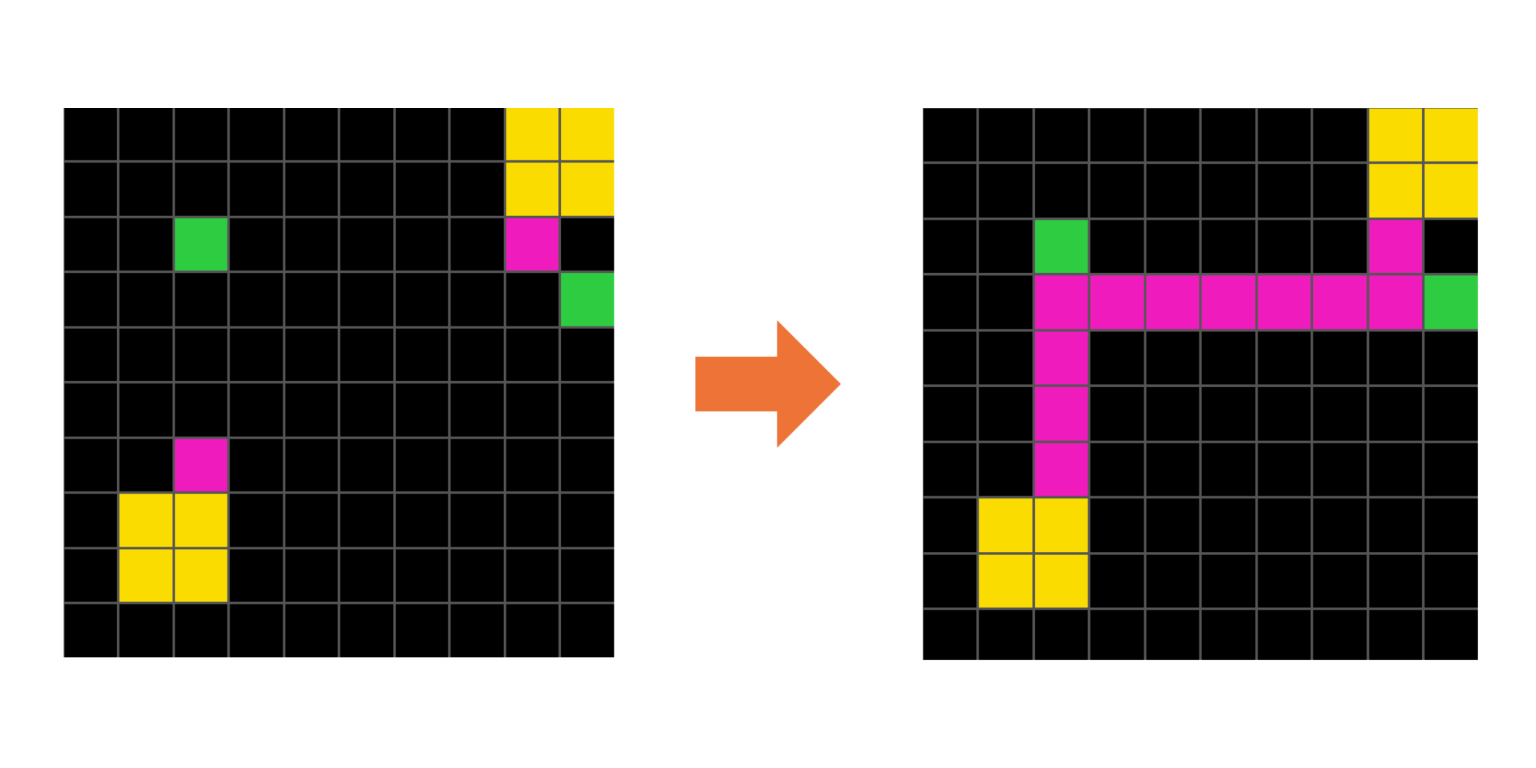
\includegraphics[width=0.6\textwidth]{Figures/1_ARC.png}
	\caption{Exemple de problème du ARC Challenge impliquant le socle de connaissance d'agentivité. }
	\label{fig:ARC}
\end{figure}



\subsection{Mesures robotiques}

Cité dans l'article de Engel: 
In a recent study [57], a simple computational model of object recognition was developed in which actions are an integral component of the perceptual process. In this model, sensorimotor contingencies (SMCs) were implemented as multistep, actioncon-ditional probabilities of future sensory observations.

\cite{maye_discrete_2011}
\cite{sanchez-fibla_acquisition_2011}

\begin{figure}[ht]
	\centering
		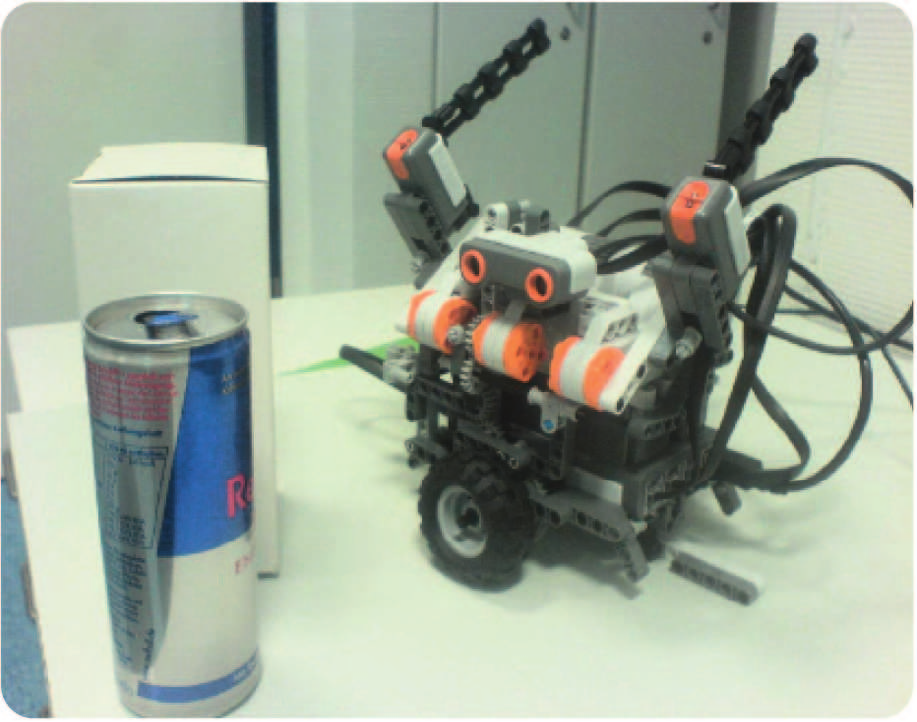
\includegraphics[width=0.4\linewidth]{Figures/1_maye_robot.png}%
	\quad
		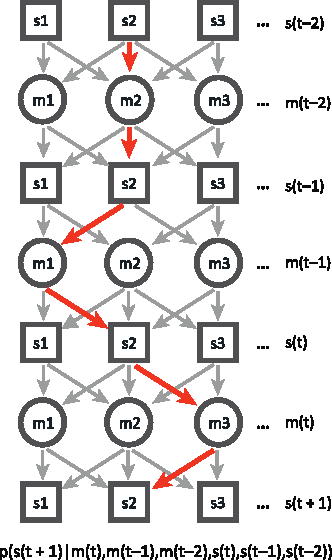
\includegraphics[width=0.18\linewidth]{Figures/1_maye_path.pdf}
	\caption{Expérimentation robotique adaptée de Engel et al. \cite[Fig.~I]{engel_wheres_2013}.
		Gauche: robot interagissant avec un objet à travers un capteur d'écho-localisation et des bras articulés.
		Droite: séquence d'expériences sensorimotrices permettant au robot de reconnaitre l'objet. 
	}
	\label{fig:maye}
\end{figure}


\subsection{Bilan des mesures}

La figure \ref{fig:mesures} résume le paysage des différentes approches pour mesurer l'intelligence. 
Ce manuscrit se situe dans le quadrant supérieur droit: les mesures dynamiques faisant appelle au jugement humain, soit par interaction directe d'un humain avec l'agent, soit par analyse des comportements basés sur des enregistrements ou des traces. 


\begin{figure}[ht]
	\centering
	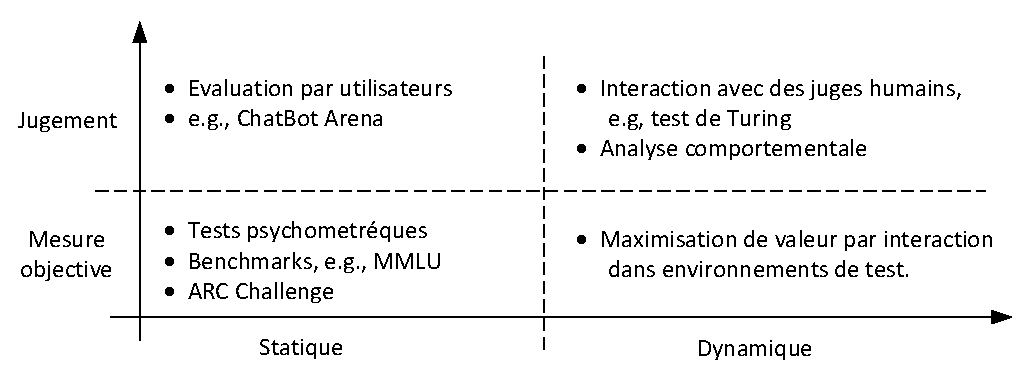
\includegraphics[width=0.8\textwidth]{Figures/1_mesures.pdf}
	\caption{Différents modes d'évaluation de l'intelligence.}
	\label{fig:mesures}
\end{figure}



\section{Conclusion}

Notre examen de l'apprentissage développemental naturel nous conduit à penser que le problème suivant est un problème intéressant en informatique:
Construire et réitérer des comportements spatio-séquentiels hiérarchiques basés sur des préférences intéractionnelles initiales
La possibilité de réiter des comportements appris à un haut niveau hiérarchique de manière adaptée implique la capacité de construire des représentations pertinentes du monde tel que l'agent enfait l'expérience. 